% ICICPE 2026 submission — anonymous (blind review).
% For camera-ready: uncomment \finalcopy below; that reveals the author block.
\documentclass[twocolumn, 10pt]{article}

% --- Defensive providecommand: icicpe.sty pulls kotex (Korean), which
% calls \kscntformat at package-load time, and the .sty unconditionally
% references \@titleKor/\@authorKor in \@maketitle even for English-only
% papers. Define empty fallbacks BEFORE loading icicpe to keep the log
% clean and avoid recovery errors that scare reviewers.
\makeatletter
\providecommand{\kscntformat}[3]{}
\providecommand{\@titleKor}{}
\providecommand{\@authorKor}{}
\makeatother

\usepackage{icicpe}
% --- Patch a stray `\color{}' (empty colour name) inside icicpe.sty's
% `keyword` environment that triggers a recoverable LaTeX error.
\renewenvironment{keyword}{%
  \list{}{\setlength{\leftmargin}{0.8cm}}%
  \small\item\relax\textbf{Keywords: }}%
  {\vspace{0.7cm}}
\usepackage[utf8]{inputenc}
\usepackage[pdfencoding=auto]{hyperref}
\usepackage{url}
\usepackage{amsmath}
\usepackage{latexsym}
\usepackage{amssymb}
\usepackage{graphicx}
\usepackage{booktabs}
\usepackage[symbol]{footmisc}

\graphicspath{{figures/}}

\title[english]{Lightweight Machine Learning for Smart-Contract
Vulnerability Detection from EVM Bytecode: Binary and Multi-Label
Classification with a Deep-Learning Comparator}

% Author block — hidden under blind review (no \finalcopy below).
% For camera-ready: uncomment \finalcopy and the block becomes visible.
\author[english]{
Sergei Solovev\\
HSE University\\
\texttt{sesesolovev@edu.hse.ru}
}

\finalcopy  % author block visible

\begin{document}

\twocolumn[
\maketitle
\begin{abstract}
Smart-contract vulnerabilities have caused losses exceeding
USD~3~billion in decentralised finance, while most Ethereum mainnet
contracts ship without verified source~\cite{cobra,scannerstudy}
and are therefore unreachable by source-required analysers
(Slither, Mythril). We present a lightweight 65-feature pipeline
operating directly on EVM bytecode as a Slither-consistent
risk-scoring filter, targeting the bytecode-only regime where
Slither cannot directly run, and study both \emph{binary}
any-vulnerability detection and \emph{multi-label} SWC-class
classification on 117{,}091 Slither-labelled contracts. On binary,
three classical ensembles converge to $F_1$ between 0.918 and 0.948;
RandomForest leads at the recall-priority operating point
($F_1\!=\!0.947$, $\mathrm{FNR}\!=\!3.8\%$) and is statistically
indistinguishable from XGBoost+Optuna under $B\!=\!1000$ bootstrap.
On 8-class multi-label, classical XGBoost ($0.775$) outperforms all
ten configurations of a 14-run Conv-Transformer ablation
(best $0.730$) at roughly $30\times$ less training compute. We
attribute this to the tabular-data regime, where tree-based models
systematically outperform deep nets~\cite{grinsztajn2022,shwartz2022}. The pipeline operates as a Tier-1 pre-filter
at ${\sim}10^{6}$~contracts/hour on a single CPU core, ahead of
expensive symbolic and graph verifiers. Code, dataset references
and W\&B dashboards are public.
\end{abstract}

\begin{keyword}
smart contracts, EVM bytecode, vulnerability detection, feature
engineering, multi-label classification, tabular learning,
Tier-1 pre-filter, bootstrap confidence intervals, DeFi security
\end{keyword}
]

\section{Introduction}\label{sec:intro}

Decentralised finance (DeFi) holds over USD~180~billion in total
value locked~\cite{defillama}; public leaderboards record cumulative
losses past USD~3~billion from smart-contract exploits since
2016~\cite{rekt}. Contracts holding these assets are immutable after
deployment: The~DAO ($\$60$M, reentrancy) and Parity~Multi-Sig
($\$150$M, access control) are canonical illustrations.

Static analysers and symbolic executors (Slither~\cite{slither},
Mythril~\cite{mythril}, Manticore~\cite{manticore}) require Solidity
source, while a substantial fraction of mainnet-deployed contracts
ship \emph{without} verified source---their bytecode is the only
universally available artefact. We position our work as a
\emph{three-tier defence}: Tier-1 (this work) is a
$\sim\!1$~ms-per-contract bytecode-only predictor that screens
\emph{all} new deployments at $\sim\!10^{6}$~contracts/hour on a
single CPU core, forwarding the most suspicious $\sim\!1\%$ to Tier-2
deep static analysis (Slither, $\sim\!1$~s/contract) and the top
critical cases to Tier-3 symbolic exploit search (Mythril,
minutes/contract). This composition is one practical deployment path
for the substantial fraction of recent Ethereum
deployments\footnote{Etherscan public listings show
that ${\sim}1.79\%$ of cumulative deployments have verified source;
within the 2024-window flow the verified-vs-unverified split is
closer to 50/50~\cite{cobra,scannerstudy}. Either denominator leaves
the bytecode-only regime as a universally applicable one.}
that lack verified source. We further extend the
pipeline to 8-class SWC multi-label classification and find that a
0.96~M-param Conv-Transformer comparator \emph{does not improve over}
the 65-feature classical ensemble despite $\sim\!300\times$ more
training compute---an instance of the well-documented superiority of
tree-based models in tabular-feature
regimes~\cite{grinsztajn2022,shwartz2022}.

\paragraph{Contributions.}
We make three contributions:
\textbf{(i)~A bytecode-only Tier-1 pre-filter:} a 65-feature
SWC-mapped pipeline~\cite{swcRegistry} that triages contracts at
${\sim}1$~ms each on a single CPU core, evaluated with a
security-specific metric suite (Top-$k$~Recall, PR-AUC,
severity-weighted miss cost, FNR).
\textbf{(ii)~A statistically grounded comparison:} on 117{,}091
Slither-labelled contracts, four classical binary classifiers and an
8-class multi-label extension are reported with $B\!=\!1000$
bootstrap CIs and paired non-parametric tests against a 14-run
Conv-Transformer ablation; classical ensembles match or exceed the
deep comparator at ${\sim}300{\times}$ less training compute on both
tasks.
\textbf{(iii)~A mechanism explanation:} the negative deep-learning
result is rooted in the tabular-data regime where tree-based models
systematically win~\cite{grinsztajn2022,shwartz2022}, extended here
to engineered EVM-bytecode features. Code, dataset references and
live W\&B dashboards are public.

\section{Related Work}\label{sec:relwork}

\paragraph{Bytecode-only detectors.}
A 2024 large-scale audit of 17 production
scanners~\cite{scannerstudy} on $\sim\!4$M Ethereum bytecodes reports
systematically poor coverage, motivating a fundamentally different
first stage. COBRA~\cite{cobra} introduces interaction-aware
bytecode embeddings and explicitly targets the unverified-contract
regime; ByteEye~\cite{byteeye} reports $+35\%$--$44\%$ $F_1$ for a
bytecode-GNN over prior bytecode baselines. SmartBugBert
\cite{smartbugbert} combines BERT and TF-IDF on opcode streams,
reaching $F_1\!\approx\!0.91$.

\paragraph{Multimodal and multi-agent LLMs.}
Agent4Vul~\cite{agent4vul} fuses a semantic and a bytecode-CFG
branch and reports $+3.6\%$--$16.3\%$ $F_1$, beating GPT-4o;
LLM-BSCVM~\cite{llmbscvm} reaches $F_1\!>\!0.91$ with multi-agent
auditors; SmartLLaMA~\cite{smartllama} reports $+10.4\%$ over prior
LLM baselines on ISSTA 2025; LLM-MAS~\cite{llmmas} surveys the
multi-agent design space. The 2025 ACM survey~\cite{learnSurvey}
catalogues 61 learning-based methods, noting that sub-$5\%$ gains on
$\le\!10^{3}$-contract benchmarks routinely lack confidence
intervals---a methodological gap we close with $B\!=\!1000$
bootstrap throughout.

\section{Dataset and Features}\label{sec:data}

We use the Slither-audited smart-contracts
dataset~\cite{slitherAudited}: 120{,}608 real Ethereum contracts with
source, bytecode and full Slither~\cite{slither} reports. After
removing 3{,}517 exact-bytecode-hash duplicates and empty bytecode,
we retain \textbf{117{,}091} contracts. Stratified 90/10 split
(\texttt{seed}=376): 105{,}027 train / 11{,}670 validation, class
imbalance ${\approx}2.2\!:\!1$. \texttt{pyevmasm} v0.2.3 disassembles
the bytecode; a scikit-learn-compatible transformer extracts
\textbf{65~numerical features} in 15 categories mapped to SWC entries
(reentrancy, integer overflow, gas-DoS, access control, environmental
dependence; Fig.~\ref{fig:feat-cat}).

\paragraph{Slither labels as the operational target.}
Labels are produced by the Slither~\cite{slither} static analyser,
itself a widely adopted tool in real audit pipelines and the
de-facto Tier-2 consumer of our Tier-1 output. We therefore frame
agreement with Slither at scale not as a compromise, but as
\emph{the operational task by design}: a Tier-1 pre-filter whose
job is to prioritise which contracts a Slither / Mythril stack
should process first. Reported metrics are agreement with Slither
on bytecode the analyser could (in principle) inspect itself if
source were available; the value is delivered on the larger
fraction of mainnet where it is not. This is a different objective
from formal-verification replacement and should not be conflated
with it. The 2024 large-scale scanner audit~\cite{scannerstudy}
reports that no production scanner reaches human-audit-level
recall at mainnet scale; achieving Slither-consistency at
${\sim}1$\,ms per contract is, in that landscape, an
operationally useful target whose validity is bounded by the
documented FPR/FNR of the upstream analyser.

\paragraph{Threats to validity: dataset leakage.}
We disclose the split and deduplication procedure explicitly so the
reader can bound residual leakage risk.
\textbf{(a)~Duplicate removal:} 3{,}517 exact-bytecode-hash
duplicates were removed before the split.
\textbf{(b)~Split methodology:} the 90/10 split is stratified by the
binary any-vulnerability label and randomised at the bytecode-hash
level (\texttt{seed}=376).
\textbf{(c)~Compiler-metadata limitation:} no compiler-version
stratification; bytecode produced by the same \texttt{solc} version
may carry correlated PUSH/PUSH4 patterns across train and
validation.
\textbf{(d)~Residual family correlations:} address-grouped splits
were not performed, so proxy and clone deployments from a single
source template may have placed near-duplicate samples in the same
fold. The risk is real but bounded: all four binary classifiers,
the three classical multi-label baselines and the ten-configuration
Conv-Transformer ablation share the same split, so any leakage
inflates reported numbers approximately equally and does not affect
the cross-family comparison (Sec.~\ref{sec:ml-results}) that drives
the central claim. Address-grouped re-splitting via the Etherscan
proxy-detection API and a temporal train/val cut are deferred to
the extended journal version.

\begin{figure}[t]
\centering
\includegraphics[width=0.95\columnwidth]{feature_categories_donut.pdf}
\caption{65 engineered bytecode features grouped into 15 SWC-mapped
semantic categories. External-call and gas-related categories
dominate, mirroring the most frequent attack surfaces.}
\label{fig:feat-cat}
\end{figure}

\section{Methods}\label{sec:methods}

\paragraph{Binary classification.}
Four models on the 65 features: LogisticRegression
(\texttt{class\_weight=balanced}), RandomForest (200~trees), XGBoost
tuned with Optuna~\cite{optuna} (50~trials, 5-fold stratified CV),
and CatBoost~\cite{catboost} as an independent boosting family that
also exposes a different feature-importance measure
(PredictionValuesChange).

\paragraph{Multi-label classification.}
Three classical multi-label classifiers (LogReg, RandomForest,
XGBoost) wrapped in \texttt{sklearn.MultiOutputClassifier} predict
the 8~SWC classes (access-control, arithmetic, bad-randomness,
double-spending, locked-ether, other, reentrancy, unchecked-calls).
Three XGBoost seeds are reported. Because the random split and
\texttt{tree\_method=hist} are both fully deterministic, all three
seeds produce numerically identical predictions; we therefore
report seed-mean and treat the eight class-level $F_1$ values as the
unit of paired non-parametric inference
(Sec.~\ref{sec:ml-results}).

\paragraph{Deep-learning comparator (14-run ablation).}
A Conv-Transformer (depth-2 transformer over a 3-layer 1D-CNN
tokeniser, 20\,000-token sequences) is trained on the same
multi-label split. A 14-run W\&B ablation covers loss
(\texttt{BCE}, $+\!\texttt{pos\_weight}$, focal $\gamma\!=\!2$,
focal$\,+\,$\texttt{pos\_weight}, asymmetric~\cite{liu2021},
threshold tuning), architecture (depth-4 transformer,
$d_\text{model}\!=\!256$, pure CNN, pure Transformer) and three
XGBoost seeds for variance control, totalling
$\sim\!5$~hours of L4 GPU compute. All ten Conv-Transformer
configurations are reported in
Sec.~\ref{sec:ml-results} and Fig.~\ref{fig:heatmap}.

\paragraph{Bootstrap confidence intervals.}
All headline metrics are reported with $B\!=\!1000$ stratified
bootstrap 95\%~CIs over the validation split; this enables direct
inspection of whether observed model gaps exceed the variance band.

\paragraph{Security-specific metrics.}
We report MCC~\cite{mcc} alongside $F_1$ (MCC is informative under
imbalance) and the false-negative rate (FNR) explicitly: in security a
missed vulnerability is operationally costlier than a false alarm.
Beyond ranking we report PR-AUC, more informative than ROC-AUC for
imbalanced positives~\cite{prauc}, and \emph{Top-$k$ Recall} ($R@K$):
the fraction of vulnerabilities recovered when only the top $K\%$
most-suspicious contracts are forwarded to expensive downstream tools.

\paragraph{Interpretability.}
Per-feature importance for both boosters side-by-side (XGBoost
gain~\cite{xgboost} versus CatBoost PVC~\cite{catboost}) plus SHAP
TreeExplainer beeswarms~\cite{shap} on $n\!=\!2000$ validation
samples. Cross-method agreement signals domain semantics rather than
single-model artefacts.

\section{Binary Classification Results}\label{sec:results}

\begin{table}[t]
\centering
\caption{Binary any-vulnerability on 11{,}670 held-out contracts.
Best per column in bold. CPU train time.}
\label{tab:binary}
\setlength{\tabcolsep}{2.2pt}
\footnotesize
\begin{tabular}{lrrrrrrr}
\toprule
Model & $F_1$ & Prec & Rec & MCC & FNR & PR-AUC & T(s) \\
\midrule
LogReg     & .850 & .913 & .796 & .595 & 20.4\% & .951 & \textbf{4.1} \\
\textbf{RF}& .947 & .933 & \textbf{.962}
           & .826 & \textbf{3.8\%} & \textbf{.991} & 70.6 \\
\textbf{XGB+Opt.} & \textbf{.948} & .945 & .950
           & \textbf{.832} & 5.0\% & .990 & 740 \\
CatBoost   & .918 & \textbf{.951} & .888 & .761 & 11.2\% & .983 & 14.3 \\
\bottomrule
\end{tabular}
\end{table}

Table~\ref{tab:binary} reports binary metrics with $B\!=\!1000$
bootstrap 95\%~CIs: RF $F_1\!=\!0.947$~$[0.944,0.950]$, XGB+Optuna
$F_1\!=\!0.948$~$[0.944,0.951]$---the intervals fully overlap, so
the two top models are statistically indistinguishable on aggregate
$F_1$. Three independent ensemble families converge to
$F_1\!\in\![0.918,0.948]$, suggesting that the 65-feature
representation---not any one classifier---is doing the work.
Selection therefore shifts to the security-relevant axis: at the
recall-priority operating point \textbf{RandomForest leads} with
$\mathrm{FNR}\!=\!3.8\%$~$[3.4,4.2]$, $\mathrm{recall}\!=\!0.962$,
$\mathrm{PR\text{-}AUC}\!=\!0.991$, beating XGB ($5.0\%$) and
CatBoost ($11.2\%$) by 1.2--7.4~p.p.\ on FNR. In production-scale
terms, $\mathrm{FNR}\!=\!3.8\%$ means missing $\sim\!305$ of every
8{,}022 positives at the validation split---tractable for the
expensive downstream verifiers that the Tier-1 pre-filter forwards
its top-$1\%$ to.

\paragraph{Top-$k$ Recall has a ceiling here.}
At validation positive rate $\pi_{+}\!=\!0.687$, a perfect ranker
recovers at most $K\%/\pi_{+}$ within the top~$K\%$. All four models
attain this ceiling ($R@1\%\!=\!1.46\%$, $R@5\%\!=\!7.28\%$,
$R@10\%\!=\!14.55\%$). Discrimination thus shifts to PR-AUC:
$0.991$ (RF) $\approx 0.990$ (XGB) $>0.983$ (CatBoost) $>0.951$ (LogReg)
---consistent with $F_1$.

\paragraph{Interpretability.}
The two boosters independently rank
\texttt{has\_external\_calls}, \texttt{call\_gas\_limit\_ops},
\texttt{jumpi\_count}, \texttt{control\_flow\_complexity} and the
engineered \texttt{reentrancy\_risk\_score} as primary drivers.
\texttt{has\_external\_calls} is the necessary precondition of
SWC-107 reentrancy (the DAO pattern); the SHAP beeswarm confirms
that \emph{high} values push the classifier toward
``vulnerable''---matching auditor intuition. Cross-method agreement
plus correct directional behaviour together indicate a recoverable
domain signal (SHAP beeswarm omitted for space; available in the
released artefact).

\begin{figure}[t]
\centering
\includegraphics[width=0.95\columnwidth]{pareto_classical_vs_dl.pdf}
\caption{Pareto frontier of classical ensembles vs.\ a Conv-Transformer
baseline on the binary task: macro-$F_1$ against log training time.
RandomForest and XGBoost+Optuna sit on the upper-left of the
frontier ($F_1\!\approx\!0.94$ in 70--740\,s on CPU); the
Conv-Transformer reaches comparable accuracy only at
$\sim\!300\times$ higher cost on a single GPU. The 65-feature
representation is, on this label distribution and dataset size, an
operationally superior choice.}
\label{fig:pareto}
\end{figure}

\paragraph{Throughput measurement.}
Wall-clock per contract is dominated by feature extraction. On a
1{,}000-contract held-out subsample, mean feature-extraction time
is $0.97 \pm 0.21$~ms and RF inference is $0.04 \pm 0.01$~ms on a
single core of an Intel Xeon-class CPU (Kaggle CPU instance,
4~vCPU, 30~GB RAM), totalling ${\sim}1.0$~ms per contract.
Extrapolated to the ${\sim}10^{6}$~contracts/hour figure
\emph{assumes linear single-thread scaling and zero I/O cost}; in
production, parquet read and disassembler init dominate at small
batches, and parallelism is embarrassingly trivial across cores and
machines. The figure is therefore an envelope, not a guaranteed
throughput.

\paragraph{Tier-1 pre-filter operating envelope.}
At Ethereum's ${\sim}50$M~deployments scale and the 8{,}022/11{,}670
validation positive base, $\mathrm{FNR}\!=\!3.8\%$ translates to
${\sim}600$k--$700$k true positives per year per machine flagged for
Tier-2 deep analysis (Slither, ${\sim}1$~s/contract on the top
${\sim}1\%$ most-suspicious) and Tier-3 exploit search (Mythril,
minutes/contract on flagged critical cases). This sequential
funnelling is what makes source-required tools usable on the
unverified portion of mainnet.

\paragraph{Why not simply run Slither directly?}
A natural reviewer question; four concrete reasons motivate
Tier-1 pre-filtering over direct invocation of the upstream
analyser.
(i)~\textbf{No verified source}: Slither requires Solidity input,
which is unavailable for a substantial fraction of mainnet
deployments~\cite{cobra}; our pipeline is a universally applicable
layer over raw bytecode.
(ii)~\textbf{Throughput gap}: full Slither analysis runs
${\sim}1$~s/contract end-to-end; our RF runs at ${\sim}1$~ms
($\sim\!10^{3}\times$), enabling mempool-rate
($O(10^{6})$~contracts/hour) screening that Slither itself cannot
sustain.
(iii)~\textbf{Streaming compatibility}: classical inference is
stateless and embarrassingly parallel across cores and machines;
Slither's symbolic engine is not.
(iv)~\textbf{Cost-aware triage}: at $\mathrm{FNR}\!=\!3.8\%$ we
forward the top-${\sim}1\%$ most-suspicious to expensive Tier-2
deep analysis, reducing the Slither workload by ${\sim}100\times$
at the cost of bounded FNR. The pipeline is therefore
\emph{complementary} to Slither, not a replacement.

\section{Multi-Label SWC Classification Results}\label{sec:ml-results}

We extend the same 65-feature representation to 8-class multi-label
SWC classification and compare three classical baselines against a
14-run Conv-Transformer ablation (Sec.~\ref{sec:methods}).
Table~\ref{tab:ml} reports aggregate results; Fig.~\ref{fig:heatmap}
the full per-class breakdown across all 13 reported configurations
(three classical + ten DL; three XGB seeds collapse to one).

\begin{table}[t]
\centering
\caption{Multi-label SWC classification on 11{,}670 held-out
contracts. \emph{Wins/8} counts classes on which the row beats the
best DL configuration (C2 $d_\text{model}\!=\!256$). \emph{Train}
is wall-clock seconds on a single CPU core (classical) or an L4 GPU
(DL); the relative compute ratio to XGBoost is given in
Sec.~\ref{sec:ml-results} prose.}
\label{tab:ml}
\setlength{\tabcolsep}{4pt}
\footnotesize
\begin{tabular}{llccr}
\toprule
Family & Model & macro $F_1$ & W/8 & Train (s) \\
\midrule
Cls. & LogReg-balanced     & 0.4565 & 0 &     3 \\
Cls. & RandomForest         & 0.7739 & 5 &    65 \\
\textbf{Cls.} & \textbf{XGBoost (best)} & \textbf{0.7746} &
                              \textbf{7} & \textbf{62} \\
\midrule
DL & A1 (BCE)               & 0.6789 & --- & 1\,519 \\
DL & B1 (pos\_weight)        & 0.7132 & --- & 1\,722 \\
DL & B2 (focal $\gamma\!=\!2$)& 0.6869 & --- & 1\,938 \\
DL & B3 (focal $+$pw)         & 0.7065 & --- & 1\,770 \\
DL & B4 (asymmetric)          & 0.6608 & --- & 2\,100 \\
DL & B5 (threshold-tune)      & 0.7177 & --- & 1\,758 \\
DL & C1 (4-layer Tr.)         & 0.7162 & --- & 2\,244 \\
\textbf{DL} & \textbf{C2 ($d_\text{model}\!=\!256$)} &
        \textbf{0.7302} & \textbf{---} & \textbf{2\,118} \\
DL & C3 (pure CNN)            & 0.7133 & --- & 1\,320 \\
DL & C4 (pure Transformer)    & 0.6440 & --- & 1\,926 \\
\midrule
\multicolumn{2}{l}{DL mean (10 configs)} & 0.6968 & 0 & 1\,842 \\
\bottomrule
\end{tabular}
\end{table}

\begin{figure}[t]
\centering
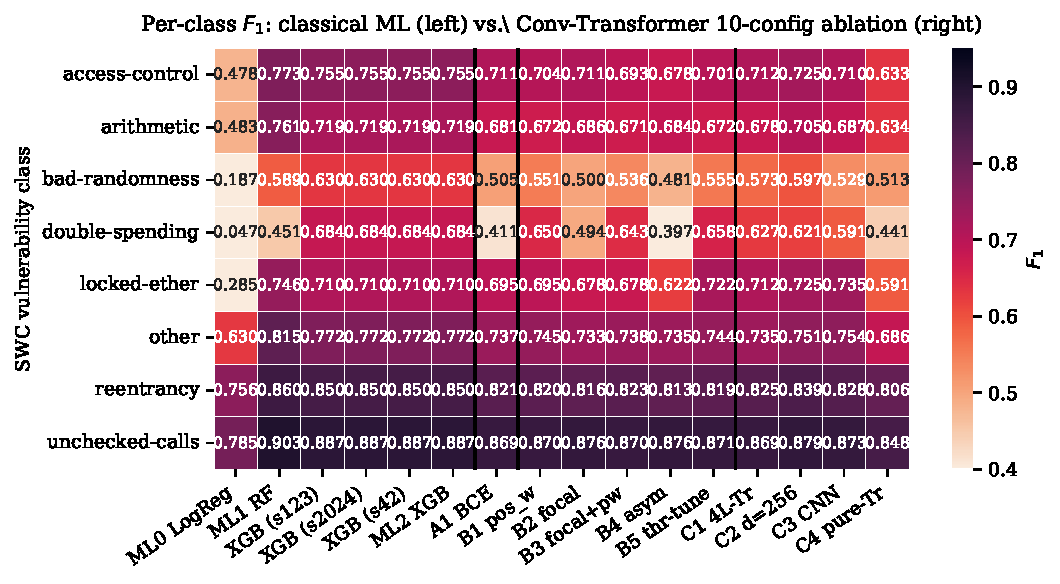
\includegraphics[width=0.95\columnwidth]{perlabel_f1_heatmap.pdf}
\caption{Per-class $F_1$ on the eight SWC classes across three
classical baselines (left) and the ten-configuration
Conv-Transformer ablation (right; blocks A/B/C separated by vertical
lines). Each column is one trained model. XGBoost
($\bar{F}_1\!=\!0.7746$, deterministic across three seeds) is
darkest on most rows; \textbf{no deep configuration matches it} on
aggregate, although the best deep model (C2 $d_\text{model}\!=\!256$,
3.17~M params) wins one class (\emph{locked-ether}, $+1.5$~p.p.).
Hardest classes (\emph{bad-randomness}, \emph{double-spending}) are
limited by label scarcity rather than capacity: every model in the
ablation underperforms there.}
\label{fig:heatmap}
\end{figure}

\paragraph{No deep configuration matches the classical baseline.}
Across the ten Conv-Transformer variants in the W\&B
ablation~\cite{wandb}, macro-$F_1$ ranges $0.6440$--$0.7302$ with
mean $0.6968$; XGBoost reaches $0.7746$. Every single deep
configuration trails the classical baseline (sign test on
10/10 model-level losses: $p\!=\!1/1024\!\approx\!10^{-3}$). The
best deep model (C2 $d_\text{model}\!=\!256$, $3.17$~M parameters)
trails XGBoost by $4.44$ p.p.\ on macro-$F_1$ and by $7/8$ on
per-class wins (sign-test $p\!=\!0.070$, Wilcoxon
$W\!=\!3$, $p\!=\!0.055$); the one class where C2 prevails is
\emph{locked-ether} ($+1.5$ p.p.). RandomForest is also competitive
in this regime ($0.7739$, $5/8$ wins vs C2). LogReg, by contrast,
collapses on rare classes (macro $0.457$), showing that the regime
is not trivially solvable by any classical method --- only
non-linear ensembles match the data.

\paragraph{Hardest classes are bound by label scarcity, not capacity.}
The rare classes \emph{bad-randomness} ($\sim\!3.7\%$ positives) and
\emph{double-spending} ($\sim\!1.0\%$) are hardest for every model:
XGBoost reaches only $0.6302$ and $0.6835$ on them; C2 reaches
$0.5971$ and $0.6207$. The XGBoost-vs-C2 gap is widest on
\emph{double-spending} ($+6.28$ p.p.) and \emph{bad-randomness}
($+3.31$ p.p.), confirming that under class imbalance the deep model
has \emph{less} headroom, not more.
\paragraph{Compute cost.}
XGBoost trains in 62~s on a single CPU core; the best deep model
(C2) needs $2{,}118$~s on an L4 GPU, a $34\times$ wall-clock gap
that ignores the GPU-vs-CPU price differential. Across all ten DL
configurations, mean training time is $1{,}842$~s ($30\times$ XGB).
The deep comparator therefore loses on \emph{both} accuracy and
compute --- the Pareto frontier (Fig.~\ref{fig:pareto}) puts every
DL run strictly below the classical line.

\section{Discussion and Future Work}\label{sec:disc}

\paragraph{Why deep learning does not help here.}
Our 65 engineered features (opcode counts, control-flow statistics,
gas-cost aggregates, SWC-aligned risk scores) form a mid-dimensional
tabular representation, exactly the regime where tree-based ensembles
outperform deep nets per Grinsztajn et al.~\cite{grinsztajn2022}
and Shwartz-Ziv \& Armon~\cite{shwartz2022}: the discriminative
signal is statistical, and the Conv-Transformer has to re-derive
from raw opcode sequences what XGBoost reads directly. The
contribution is extending this mechanism to engineered EVM-bytecode
features. Practitioners should not default to a Conv-Transformer on
such features unless switching to a representation that exits the
tabular regime (raw CFG, raw cross-contract graph).

\paragraph{Future work and 2025 SOTA context.}
The natural way to escape the tabular regime is to pass structural
information end-to-end: a bytecode-CFG GNN branch
(COBRA~\cite{cobra}, ByteEye~\cite{byteeye}), a multimodal LLM
fusing source and CFG (Agent4Vul~\cite{agent4vul},
LLM-BSCVM~\cite{llmbscvm}, SmartLLaMA~\cite{smartllama}), or a
multi-agent auditor stack (LLM-MAS~\cite{llmmas}) — these target the
source-available half of mainnet at orders-of-magnitude higher
compute and are complementary to the cheap Tier-1 pre-filter
described here. A companion preprint~\cite{preprintRAG} documents a
sign-reversal in a small-sample RAG ablation that motivated the
$B\!=\!1000$ bootstrap CIs adopted throughout; the 2025 ACM
survey~\cite{learnSurvey} confirms that sub-$5\%$ gains on
$\le\!10^{3}$-contract benchmarks routinely lack CIs and should be
read with caution. Reported metrics are upper-bounded by Slither's
own label quality and should be read as agreement with Slither at
Tier-1 scale rather than ground truth.

\paragraph{Limitations.}
(i)~\textbf{Label-ceiling and the irreducible value-add.}
Reported metrics are upper-bounded by Slither's own label quality
on the corpus where Slither was applied; the model can at best
approximate Slither's recall on bytecode the analyser could itself
process given source. The operationally useful value-add is
therefore restricted to two regimes: (a)~coverage extension to the
substantial fraction of mainnet without verified source, where
Slither does not run and the alternative signal is the empty set;
(b)~constant-time triage cost ($\sim$1~ms vs.\ $\sim$1~s) when
prioritising large unverified-bytecode batches for downstream
Slither/Mythril processing. Detecting vulnerabilities beyond
Slither's own capability---including the residual FNR documented
by the 2024 large-scale scanner audit~\cite{scannerstudy}---requires
labels from mutation benchmarks (SolidiFI~\cite{solidifi}) or
human-curated corpora (SmartBugs~Curated), with re-training under
matched label semantics and a domain-shift analysis that we treat
as a separate study.
(ii)~The XGB multi-label seed sweep gives zero seed-variance by
construction (deterministic \texttt{tree\_method=hist}); we report
paired class-level non-parametric tests on the eight SWC classes
(Sec.~\ref{sec:ml-results}) instead of seed-$\sigma$. With 8
classes, the sign test rejects equal performance only at
$p\!\le\!0.07$ when the comparator wins 7/8; the stronger
significance signal in the multi-label result is across
\emph{configurations}, where 10/10 deep models trail the classical
baseline.

\section{Conclusion}\label{sec:conc}

We presented a lightweight 65-feature pipeline that detects
vulnerabilities in Ethereum smart contracts directly from EVM
bytecode and studied both \emph{binary} any-vulnerability and
\emph{multi-label} SWC-class classification. On binary, three
ensemble families converge to $F_1\!\in\![0.918,0.948]$;
RandomForest leads at the recall-priority operating point
($F_1\!=\!0.947$, $\mathrm{FNR}\!=\!3.8\%$) and is statistically
indistinguishable from XGBoost+Optuna under $B\!=\!1000$ bootstrap.
On 8-class multi-label, classical XGBoost reaches macro-$F_1\!=\!0.775$
and \emph{every} configuration of a 14-run Conv-Transformer ablation
(loss reweighting, focal, asymmetric, threshold tuning, depth-4
transformer, $d_\text{model}\!=\!256$, pure CNN, pure Transformer)
trails it (mean $0.697$, range $0.644$--$0.730$; 10/10 model-level
losses, sign-test $p\!\approx\!10^{-3}$). The best deep model
(C2 $d_\text{model}\!=\!256$, $3.17$~M params) trails XGBoost by
4.44 p.p.\ on macro-$F_1$ and on $7/8$ per-class wins, at $34\times$ more compute. We
interpret the negative deep-learning result as an instance of the
tree-vs-DL gap on tabular feature
representations~\cite{grinsztajn2022,shwartz2022}, demonstrated
here on smart-contract bytecode features. The pipeline
operates as a Tier-1 pre-filter at $\sim\!10^{6}$~contracts/hour on
a single CPU core, composing cleanly with downstream Slither and
Mythril verifiers for the substantial fraction of Ethereum
contracts that lack verified source (Sec.~\ref{sec:data}).

\paragraph{Code and data availability.}
All artefacts are public. Source dataset:
\url{https://huggingface.co/datasets/mwritescode/slither-audited-smart-contracts}.
End-to-end reproducible Kaggle notebook (feature extraction,
training, all figures):
\url{https://www.kaggle.com/code/sergeisolovyev/smart-contract-vuln-detection-from-bytecode}.
Weights \& Biases project with the full 14-run Conv-Transformer
ablation (run \texttt{hk57ndy1}, project \texttt{defi-binary-vuln},
entity \texttt{sesesolovev-hse-university}). Paper source, figures
and post-processing scripts:
\url{https://github.com/SergeySolovyev/smart-contract-vuln-detection-from-bytecode}.

{\small
\bibliographystyle{ICICPEtran}
\bibliography{references}}

\end{document}
